% The eval chain of klayout/drc/adk_assembly.drc.
% One Ruby string, evaluated once. The conditional segments are bracketed on
% the right so the additivity of the interconnect axis is visible.
\documentclass[border=4pt]{standalone}
\usepackage{tikz}
\usetikzlibrary{arrows.meta, positioning, calc, decorations.pathreplacing}
\usepackage[T1]{fontenc}
\usepackage{lmodern}

\definecolor{IHPfg}{RGB}{0,80,139}
\definecolor{IHPaccent}{RGB}{109,112,114}
\definecolor{cValid}{RGB}{210,80,80}

\newcommand{\adkT}[1]{\texttt{#1}}
% Figure labels are short. Never hyphenate them.
\newcommand{\adkNoHyph}{\hyphenpenalty=10000\exhyphenpenalty=10000}

\begin{document}
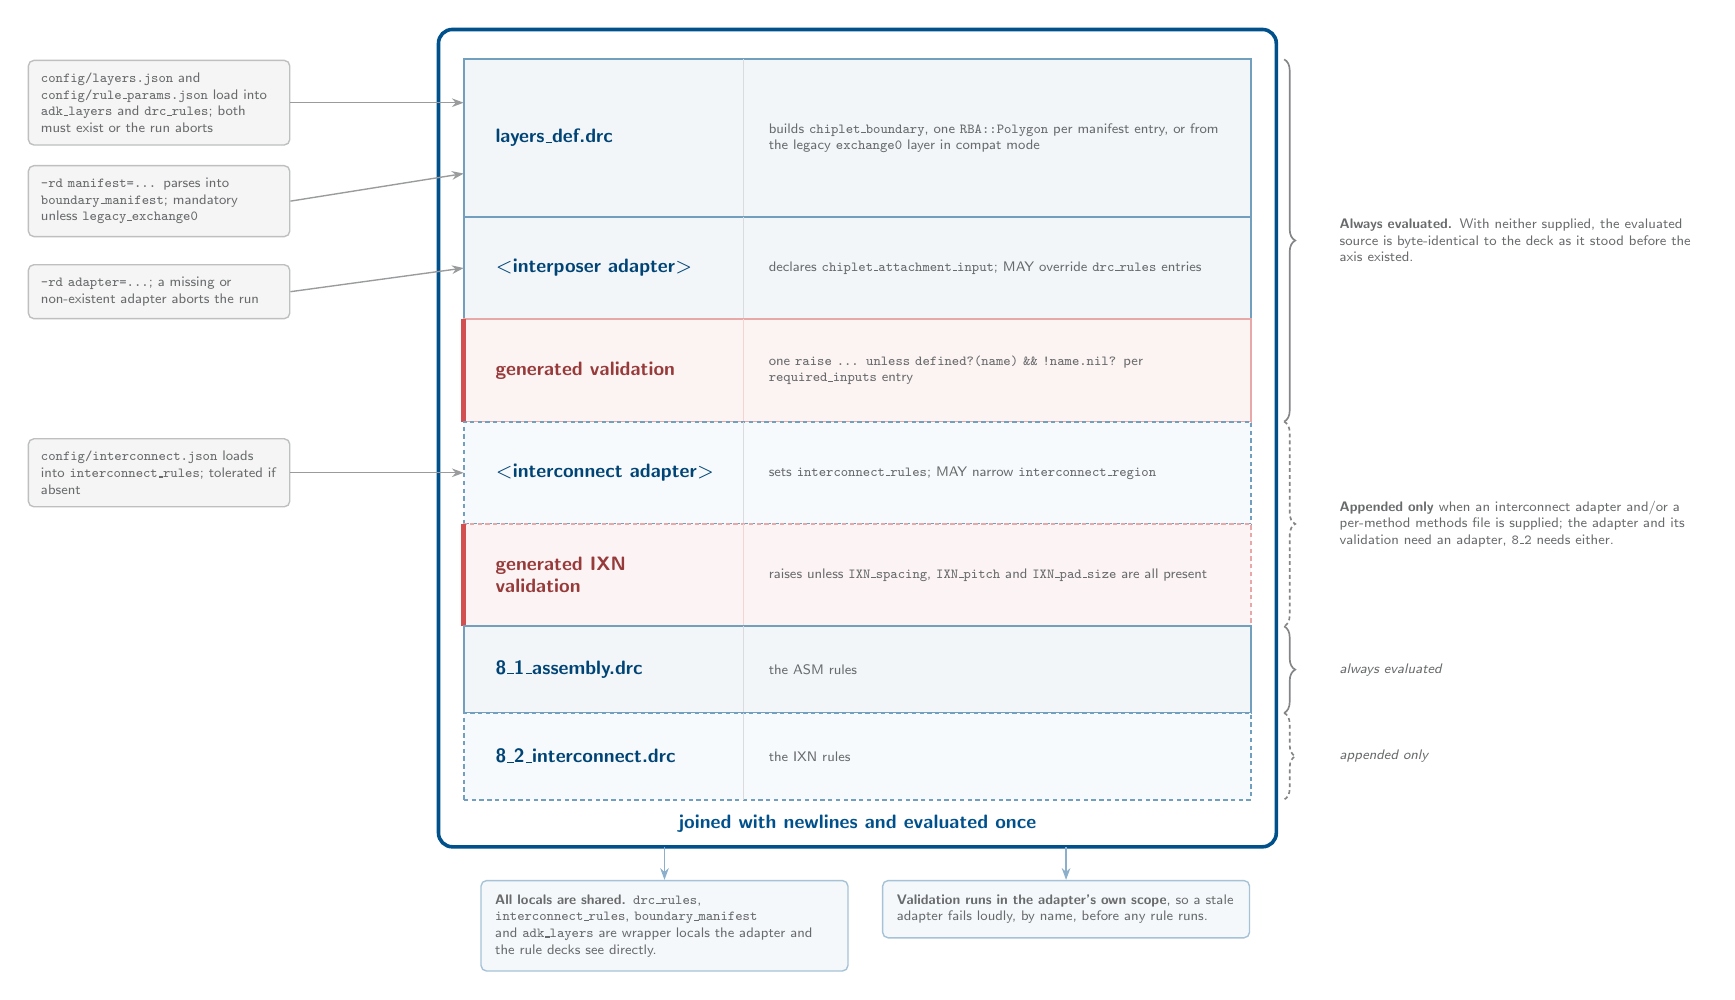
\begin{tikzpicture}[
    >=Stealth,
    adkname/.style={
        anchor=west, align=left, text width=3.10cm,
        font=\sffamily\scriptsize\bfseries, text=IHPfg!85!black
    },
    adknamev/.style={
        anchor=west, align=left, text width=3.10cm,
        font=\sffamily\scriptsize\bfseries, text=cValid!72!black
    },
    adkdesc/.style={
        anchor=west, align=left, text width=5.95cm,
        font=\sffamily\tiny\adkNoHyph, text=IHPaccent!95!black
    },
    adkcard/.style={
        rectangle, rounded corners=2pt,
        draw=IHPaccent!45, fill=IHPaccent!7, line width=0.5pt,
        anchor=east, align=left, text width=3.00cm, inner sep=1.6mm,
        font=\sffamily\tiny\adkNoHyph, text=IHPaccent!95!black
    },
    adkarrow/.style={
        -{Stealth[length=1.5mm, width=1.1mm]}, line width=0.5pt, color=IHPaccent!70
    },
    adkbrace/.style={
        decorate, decoration={brace, amplitude=4pt},
        line width=0.6pt, color=IHPaccent!85
    },
    adkbracec/.style={
        decorate, decoration={brace, amplitude=4pt},
        line width=0.6pt, color=IHPaccent!85, dash pattern=on 1.4pt off 1.1pt
    },
    adklbl/.style={
        anchor=west, align=left, text width=4.55cm,
        font=\sffamily\tiny\adkNoHyph, text=IHPaccent!95!black
    },
    adknote/.style={
        rectangle, rounded corners=2pt,
        draw=IHPfg!35, fill=IHPfg!4, line width=0.5pt,
        anchor=north, align=left, text width=4.30cm, inner sep=1.8mm,
        font=\sffamily\tiny\adkNoHyph, text=IHPaccent!95!black
    }
]

% ---------------------------------------------------------------- geometry --
\def\XL{0}        % stack left edge
\def\XR{10}       % stack right edge
\def\XS{3.55}     % name / description separator
\def\XN{0.28}     % name column
\def\XD{3.75}     % description column
\def\XB{10.42}    % brace column
\def\XT{11.00}    % brace label column

% Slab bands, top to bottom.
\def\ya{0}        \def\yb{-2.00}   % 1 layers_def.drc
\def\yc{-3.30}                     % 2 interposer adapter
\def\yd{-4.60}                     % 3 generated validation
\def\ye{-5.90}                     % 4 interconnect adapter
\def\yf{-7.20}                     % 5 generated IXN validation
\def\yg{-8.30}                     % 6 8_1_assembly.drc
\def\yh{-9.40}                     % 7 8_2_interconnect.drc

\def\yFtop{0.38}
\def\yFbot{-10.00}

% ------------------------------------------------------------- outer frame --
\draw[rounded corners=5pt, draw=IHPfg, line width=1.3pt]
    (-0.32, \yFtop) rectangle (10.32, \yFbot);
\node[font=\sffamily\scriptsize\bfseries, text=IHPfg, anchor=center]
    at (5, -9.71) {joined with newlines and evaluated once};

% ------------------------------------------------------------------- slabs --
% 1 -- layers_def.drc
\draw[draw=IHPfg!55, fill=IHPfg!5, line width=0.7pt] (\XL,\yb) rectangle (\XR,\ya);
\draw[draw=IHPaccent!25, line width=0.3pt] (\XS,\yb) -- (\XS,\ya);
\node[adkname] at (\XN, -1.00) {layers\_def.drc};
\node[adkdesc] at (\XD, -1.00) {builds \adkT{chiplet\_boundary}, one
    \adkT{RBA::Polygon} per manifest entry, or from the legacy
    \adkT{exchange0} layer in compat mode};

% 2 -- interposer adapter
\draw[draw=IHPfg!55, fill=IHPfg!5, line width=0.7pt] (\XL,\yc) rectangle (\XR,\yb);
\draw[draw=IHPaccent!25, line width=0.3pt] (\XS,\yc) -- (\XS,\yb);
\node[adkname] at (\XN, -2.65) {\textless{}interposer adapter\textgreater{}};
\node[adkdesc] at (\XD, -2.65) {declares \adkT{chiplet\_attachment\_input};
    MAY override \adkT{drc\_rules} entries};

% 3 -- generated validation
\draw[draw=cValid!50, fill=cValid!7, line width=0.7pt] (\XL,\yd) rectangle (\XR,\yc);
\draw[draw=cValid, line width=1.8pt] (\XL,\yd) -- (\XL,\yc);
\draw[draw=cValid!25, line width=0.3pt] (\XS,\yd) -- (\XS,\yc);
\node[adknamev] at (\XN, -3.95) {generated validation};
\node[adkdesc] at (\XD, -3.95) {one \adkT{raise ... unless defined?(name) \&\&
    !name.nil?} per \adkT{required\_inputs} entry};

% 4 -- interconnect adapter (conditional)
\draw[draw=IHPfg!55, fill=IHPfg!3, line width=0.7pt, dash pattern=on 1.6pt off 1.2pt]
    (\XL,\ye) rectangle (\XR,\yd);
\draw[draw=IHPaccent!25, line width=0.3pt] (\XS,\ye) -- (\XS,\yd);
\node[adkname] at (\XN, -5.25) {\textless{}interconnect adapter\textgreater{}};
\node[adkdesc] at (\XD, -5.25) {sets \adkT{interconnect\_rules}; MAY narrow
    \adkT{interconnect\_region}};

% 5 -- generated IXN validation (conditional)
\draw[draw=cValid!50, fill=cValid!6, line width=0.7pt, dash pattern=on 1.6pt off 1.2pt]
    (\XL,\yf) rectangle (\XR,\ye);
\draw[draw=cValid, line width=1.8pt] (\XL,\yf) -- (\XL,\ye);
\draw[draw=cValid!25, line width=0.3pt] (\XS,\yf) -- (\XS,\ye);
\node[adknamev] at (\XN, -6.55) {generated IXN\\validation};
\node[adkdesc] at (\XD, -6.55) {raises unless \adkT{IXN\_spacing},
    \adkT{IXN\_pitch} and \adkT{IXN\_pad\_size} are all present};

% 6 -- 8_1_assembly.drc
\draw[draw=IHPfg!55, fill=IHPfg!5, line width=0.7pt] (\XL,\yg) rectangle (\XR,\yf);
\draw[draw=IHPaccent!25, line width=0.3pt] (\XS,\yg) -- (\XS,\yf);
\node[adkname] at (\XN, -7.75) {8\_1\_assembly.drc};
\node[adkdesc] at (\XD, -7.75) {the ASM rules};

% 7 -- 8_2_interconnect.drc (conditional)
\draw[draw=IHPfg!55, fill=IHPfg!3, line width=0.7pt, dash pattern=on 1.6pt off 1.2pt]
    (\XL,\yh) rectangle (\XR,\yg);
\draw[draw=IHPaccent!25, line width=0.3pt] (\XS,\yh) -- (\XS,\yg);
\node[adkname] at (\XN, -8.85) {8\_2\_interconnect.drc};
\node[adkdesc] at (\XD, -8.85) {the IXN rules};

% ------------------------------------------------------------------ inputs --
\node[adkcard] (ca) at (-2.20, -0.55) {\adkT{config/layers.json} and
    \adkT{config/rule\_params.json} load into \adkT{adk\_layers} and
    \adkT{drc\_rules}; both must exist or the run aborts};
\node[adkcard] (cb) at (-2.20, -1.80) {\adkT{-rd manifest=...} parses into
    \adkT{boundary\_manifest}; mandatory unless \adkT{legacy\_exchange0}};
\node[adkcard] (cc) at (-2.20, -2.95) {\adkT{-rd adapter=...}; a missing or
    non-existent adapter aborts the run};
\node[adkcard] (cd) at (-2.20, -5.25) {\adkT{config/interconnect.json} loads
    into \adkT{interconnect\_rules}; tolerated if absent};

\draw[adkarrow] (ca.east) -- (\XL, -0.55);
\draw[adkarrow] (cb.east) -- (\XL, -1.45);
\draw[adkarrow] (cc.east) -- (\XL, -2.65);
\draw[adkarrow] (cd.east) -- (\XL, -5.25);

% ------------------------------------------------------------------ braces --
% Always-evaluated group: slabs 1, 2, 3 and 6.
\draw[adkbrace]  (\XB, \ya) -- (\XB, \yd);
\draw[adkbrace]  (\XB, \yf) -- (\XB, \yg);
% Conditional group: slabs 4, 5 and 7.
\draw[adkbracec] (\XB, \yd) -- (\XB, \yf);
\draw[adkbracec] (\XB, \yg) -- (\XB, \yh);

\node[adklbl] at (\XT, -2.30) {\textbf{\textcolor{IHPaccent!95!black}{Always
    evaluated.}} With neither supplied, the evaluated source is byte-identical
    to the deck as it stood before the axis existed.};
\node[adklbl] at (\XT, -5.90) {\textbf{\textcolor{IHPaccent!95!black}{Appended
    only}} when an interconnect adapter and/or a per-method methods file is
    supplied; the adapter and its validation need an adapter, \adkT{8\_2} needs
    either.};

\node[adklbl, font=\sffamily\tiny\itshape] at (\XT, -7.75) {always evaluated};
\node[adklbl, font=\sffamily\tiny\itshape] at (\XT, -8.85) {appended only};

% ------------------------------------------------------------ consequences --
\node[adknote] (na) at (2.55, -10.42) {\textbf{All locals are shared.}
    \adkT{drc\_rules}, \adkT{interconnect\_rules}, \adkT{boundary\_manifest}
    and \adkT{adk\_layers} are wrapper locals the adapter and the rule decks
    see directly.};
\node[adknote] (nb) at (7.65, -10.42) {\textbf{Validation runs in the adapter's
    own scope}, so a stale adapter fails loudly, by name, before any rule
    runs.};

\draw[adkarrow, color=IHPfg!45] (2.55, \yFbot) -- (2.55, -10.42);
\draw[adkarrow, color=IHPfg!45] (7.65, \yFbot) -- (7.65, -10.42);

\end{tikzpicture}
\end{document}
